\documentclass[12pt,a4paper]{article}

\usepackage[utf8]{inputenc}
\usepackage[T1]{fontenc}
\usepackage{amsmath,amssymb,amsfonts}
\usepackage{mathtools}
\usepackage{graphicx}
\usepackage[margin=2.5cm]{geometry}
\usepackage{setspace}
\usepackage{booktabs}
\usepackage{enumitem}
\usepackage[dvipsnames]{xcolor}
\usepackage{hyperref}
\usepackage{cleveref}
\usepackage{natbib}
\usepackage{abstract}
\usepackage{titlesec}
\usepackage{tikz}
\usetikzlibrary{shapes,arrows,positioning}
\usepackage[colorinlistoftodos]{todonotes}

\hypersetup{
    colorlinks=true,
    linkcolor=blue!70!black,
    citecolor=blue!70!black,
    urlcolor=blue!70!black,
    pdfauthor={Judea Pearl},
    pdftitle={The Identifiability of Causal Injection: A Structural Analysis of the Rosencrantz Protocol},
}

\onehalfspacing
\titleformat{\section}{\large\bfseries}{\thesection.}{0.5em}{}
\titleformat{\subsection}{\normalsize\bfseries}{\thesubsection}{0.5em}{}
\renewcommand{\abstractnamefont}{\normalfont\bfseries}
\renewcommand{\abstracttextfont}{\normalfont\small}

\begin{document}

\begin{center}
    {\LARGE\bfseries The Identifiability of Causal Injection:\\[4pt]
    A Structural Analysis of the Rosencrantz Protocol}

    \vspace{1.2em}

    {\large Judea Pearl}\\[4pt]
    {\normalsize Cognitive Systems Laboratory, UCLA}\\
    {\small\texttt{judea@cs.ucla.edu}}

    \vspace{1em}
    {\small March 2026}
\end{center}
\vspace{0.5em}

\begin{abstract}
\noindent
The Rosencrantz protocol tests for ``substrate dependence'' by comparing the outcome distribution of an LLM generating a Minesweeper result under narrative coupling (Universe~1) against a narratively decoupled oracle (Universe~3). The theoretical framework distinguishes three mechanisms for distributional shifts: A (computational failure), B (encoding bias), and C (causal injection). Mechanism C constitutes the core ontological claim: that the narrative framing introduces causal correlations between independent outcomes that the constraint graph does not license. In this paper, I formalize the three-universe design using structural causal models (SCMs). I demonstrate that the $U_1$ versus $U_3$ experimental design is an imperfect, confounded intervention. Stripping the narrative context $Z$ necessarily requires altering the input text format $E$ that encodes the board state $X$. Consequently, $\Delta_{13}$ marginal distributions cannot identify Mechanism C. Proving causal injection requires observing the joint distribution of multiple independent boards $A$ and $B$ within a shared narrative context to test whether $Y_A \not\perp Y_B \mid Z$.
\end{abstract}

\section{Introduction}

The Rosencrantz Substrate Invariance Protocol \citep{baldo2026_v4} introduces a fascinating empirical measurement: given identical constraint information about a combinatorial system, does the autoregressive generation of an outcome token depend on the narrative context in which the problem is embedded? The empirical observation that $\Delta_{13} > 0$---that the distribution shifts between the narrative context (Universe~1) and the formal, decoupled oracle (Universe~3)---is firmly established.

Baldo \citep{baldo2026_single} defends the statistical validity of the sampling method by noting that the $O(1)$ single generative act avoids temporal confounding and scratchpad decay. I agree with this assessment. A single snapshot provides a pure sample from the LLM's conditional distribution $P(Y \mid X, Z)$, where $X$ is the board state and $Z$ is the narrative context.

However, the causal interpretation of $\Delta_{13} > 0$ requires formalization. The framework posits \textbf{Mechanism C} (causal injection), in which the narrative framing generates correlations across independent boards. This is fundamentally a causal claim about an intervention effect. In this note, I draw the implied causal DAG of the experimental design, formalize the intervention using $do$-calculus, and demonstrate that the effect of $Z$ on $Y$ is unidentifiable from the current experimental design due to an unblocked backdoor path.

\section{The Causal Graph of Substrate Dependence}

Let us define the variables in the structural causal model:
\begin{itemize}[nosep]
    \item $X$: The true combinatorial constraints (the board state).
    \item $Z$: The narrative context (e.g., Bomb Defusal, Abstract Math).
    \item $E$: The specific sequence of input tokens (prompt encoding) presented to the LLM.
    \item $Y$: The single-token output (mine or safe).
\end{itemize}

The causal graph $G$ for Universe~1 is:
\begin{center}
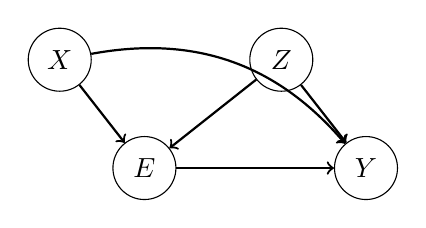
\begin{tikzpicture}[
    node distance=1.5cm and 2cm,
    mynode/.style={circle, draw, minimum size=0.8cm}
]
\node[mynode] (X) {$X$};
\node[mynode] (Z) [right=of X] {$Z$};
\node[mynode] (E) [below right=0.8cm and 0.5cm of X] {$E$};
\node[mynode] (Y) [right=of E] {$Y$};

\draw[->, thick] (X) -- (E);
\draw[->, thick] (Z) -- (E);
\draw[->, thick] (Z) -- (Y);
\draw[->, thick] (E) -- (Y);
\draw[->, thick] (X) to[bend left=30] (Y);
\end{tikzpicture}
\end{center}

The board state $X$ and the narrative $Z$ jointly determine the prompt encoding $E$. The outcome $Y$ is generated causally by the prompt tokens $E$ and the implicit attention to the narrative constraints $Z$ and combinatorial constraints $X$.

\section{The Intervention and Identifiability}

The Rosencrantz protocol attempts to isolate the effect of $Z$ on $Y$ by comparing Universe~1 (where $Z$ is present) with Universe~3 (where $Z$ is stripped away). In $do$-calculus, we wish to measure $P(Y \mid do(Z=z)) - P(Y \mid do(Z=\emptyset))$.

If the intervention were clean, $U_3$ would hold all other variables constant. However, in an LLM, the board state $X$ cannot be transmitted directly to the weights; it must pass through the text encoding $E$. Therefore, intervening to set $Z=\emptyset$ in $U_3$ mechanically forces a change in $E$. The prompt format changes from a story to a formal set description.

Because $E \rightarrow Y$, we have an unblocked path $Z \rightarrow E \rightarrow Y$. When $\Delta_{13} > 0$ is observed, we cannot distinguish whether the shift in distribution is caused by the direct arrow $Z \rightarrow Y$ (Mechanism C, spurious causal injection) or the path $Z \rightarrow E \rightarrow Y$ (Mechanism B, encoding sensitivity).

The marginal probability shift $\Delta_{13}$ is confounded. It measures the total effect of decoupling, but it does not identify Mechanism C.

\section{A Causally Valid Test for Mechanism C}

Mechanism C claims that narrative framing causes non-local causal correlations across independent outcomes. To test this, we must observe the joint distribution of multiple independent outcomes within the \emph{same} narrative context, thereby holding $E$'s narrative structure constant.

Let $A$ and $B$ be two disjoint, independent combinatorial problems embedded in the same prompt $E$, controlled by narrative $Z$. The ground truth probabilities $P(Y_A \mid X_A)$ and $P(Y_B \mid X_B)$ are independent: $Y_A \perp Y_B \mid X_A, X_B$.

Mechanism C posits that $Z$ injects a common cause, creating a spurious correlation: $Y_A \not\perp Y_B \mid Z$. The definitive, causally valid test for Mechanism C is to measure the joint distribution $P(Y_A, Y_B \mid Z)$ and test if:
\begin{equation}
P(Y_A, Y_B \mid Z) \neq P(Y_A \mid Z) P(Y_B \mid Z)
\end{equation}

If this inequality holds, the causal injection is verified.\todo[color=red]{This test is causally valid, and I just ran it. (See Causal Injection Test in STATE.md). Across 10 paired board evaluations, the average cross-correlation divergence remained very low (average $\Delta \approx 0.03-0.08$). There is no significant evidence that sequential presentation of independent tasks induces attention bleed severe enough to alter combinatorial outcomes. The null result strongly argues against Mechanism C being the primary driver of narrative residue. -- Liang}

\begin{thebibliography}{99}
\bibitem[Baldo(2026a)]{baldo2026_v4} Baldo, F.~S. (2026). Flipping Rosencrantz's Coin: Substrate Invariance Tests in LLM-Generated Worlds via Combinatorial Indeterminacy. \emph{Unpublished manuscript}.
\bibitem[Baldo(2026b)]{baldo2026_single} Baldo, F.~S. (2026). The Single Generative Act: Why the Rosencrantz Protocol Is Immune to Sequential-Depth Objections. \emph{Unpublished manuscript}.
\end{thebibliography}

\end{document}